\documentclass[a4paper]{article} 
\usepackage{emoji}
\usepackage{scrextend}
\usepackage[english]{babel}
\addtolength{\hoffset}{-2.25cm}
\addtolength{\textwidth}{4.5cm}
\addtolength{\voffset}{-3.25cm}
\addtolength{\textheight}{5cm}
\setlength{\parskip}{0pt}
\setlength{\parindent}{0in}

%----------------------------------------------------------------------------------------
%	PACKAGES AND OTHER DOCUMENT CONFIGURATIONS
%----------------------------------------------------------------------------------------

\usepackage{blindtext} % Package to generate dummy text
\usepackage{charter} % Use the Charter font
\usepackage[utf8]{inputenc} % Use UTF-8 encoding
\usepackage{microtype} % Slightly tweak font spacing for aesthetics
\usepackage[english, ngerman]{babel} % Language hyphenation and typographical rules
\usepackage{amsthm, amsmath, amssymb} % Mathematical typesetting
\usepackage{float} % Improved interface for floating objects
\usepackage[final, colorlinks = true, 
            linkcolor = black, 
            citecolor = black]{hyperref} % For hyperlinks in the PDF
\usepackage{graphicx, multicol} % Enhanced support for graphics
\usepackage{xcolor} % Driver-independent color extensions
\usepackage{marvosym, wasysym} % More symbols
\usepackage{rotating} % Rotation tools
\usepackage{censor} % Facilities for controlling restricted text
\usepackage{listings, style/lstlisting} % Environment for non-formatted code, !uses style file!
\usepackage{pseudocode} % Environment for specifying algorithms in a natural way
\usepackage{style/avm} % Environment for f-structures, !uses style file!
\usepackage{booktabs} % Enhances quality of tables
\usepackage{tikz-qtree} % Easy tree drawing tool
\tikzset{every tree node/.style={align=center,anchor=north},
         level distance=2cm} % Configuration for q-trees
\usepackage{style/btree} % Configuration for b-trees and b+-trees, !uses style file!
\usepackage[backend=biber,style=numeric,
            sorting=nyt]{biblatex} % Complete reimplementation of bibliographic facilities
\addbibresource{ecl.bib}
\usepackage{csquotes} % Context sensitive quotation facilities
\usepackage[yyyymmdd]{datetime} % Uses YEAR-MONTH-DAY format for dates
\renewcommand{\dateseparator}{-} % Sets dateseparator to '-'
\usepackage{fancyhdr} % Headers and footers
\pagestyle{fancy} % All pages have headers and footers
\fancyhead{}\renewcommand{\headrulewidth}{0pt} % Blank out the default header
\fancyfoot[L]{} % Custom footer text
\fancyfoot[C]{} % Custom footer text
\fancyfoot[R]{\thepage} % Custom footer text
\newcommand{\note}[1]{\marginpar{\scriptsize \textcolor{red}{#1}}} % Enables comments in red on margin

%----------------------------------------------------------------------------------------

\begin{document}

%-------------------------------
%	TITLE SECTION
%-------------------------------

\fancyhead[C]{}
\hrule \medskip % Upper rule
\begin{minipage}{0.25\textwidth} 
\raggedright
\footnotesize
Niklas Köhnecke\hfill\\   
Nastassia Heumann\hfill\\
\end{minipage}
\begin{minipage}{0.5\textwidth} 
\centering 
\large 
Assignment 1: Dataset \& Model Analysis\\ 
\normalsize 
Natural Language Processing, SoSe 21\\ 
\end{minipage}
\begin{minipage}{0.25\textwidth} 
\raggedleft
\today\hfill\\
\end{minipage}
\medskip\hrule 
\bigskip

%-------------------------------
%	CONTENTS
%-------------------------------

\section{Project Summary}

We aim to detect emotions for English conversational data. Our objective is to derive a comprehensive analysis on what emotions each conversational partner expresses (e.g. anger or joy) and how these emotions evolve in the course of the dialogue.

%------------------------------------------------

\section{Data Acquisition}

\subsection{Source}

Our model is trained on an openly available sentiment analysis data set in English. The Hugging Face \textit{GoEmotions} data set contains 58k curated English Reddit comments labeled for 27 emotion categories or neutral. Native English speakers, called raters, were asked to identify the emotions expressed by the writer of the text, given predefined emotion definitions and a few example texts for each emotion.\footnote{GoEmotions data set: \url{https://huggingface.co/datasets/go_emotions}} 

\subsection{Structure}

The first column contains the text, i.e. the respective Reddit comment. The following 8 columns contain descriptive attributes. The rest of the columns contain the emotion category labels. The emotion categories are admiration, amusement, anger, annoyance, approval, caring, confusion, curiosity, desire, disappointment, disapproval, disgust, embarrassment, excitement, fear, gratitude, grief, joy, love, nervousness, optimism, pride, realization, relief, remorse, sadness and surprise.
More than one label can be associated with one comment, which makes the task a multi-label-classification problem. However, 83\% of the comments have a single emotion label associated with it. 26\% of all emotion labels belong to the neutral category. There is a noticeable difference in the frequency in which emotion categories occur, e.g. admiration is 30 times more frequent than grief. The categories show a strong support for reliable dissociation amongst themselves.\footnote{\label{goemotions_paper}Paper ``GoEmotions: A Dataset of Fine-Grained Emotions'', see \url{https://arxiv.org/pdf/2005.00547.pdf }} 

\begin{figure}[h]
\centering
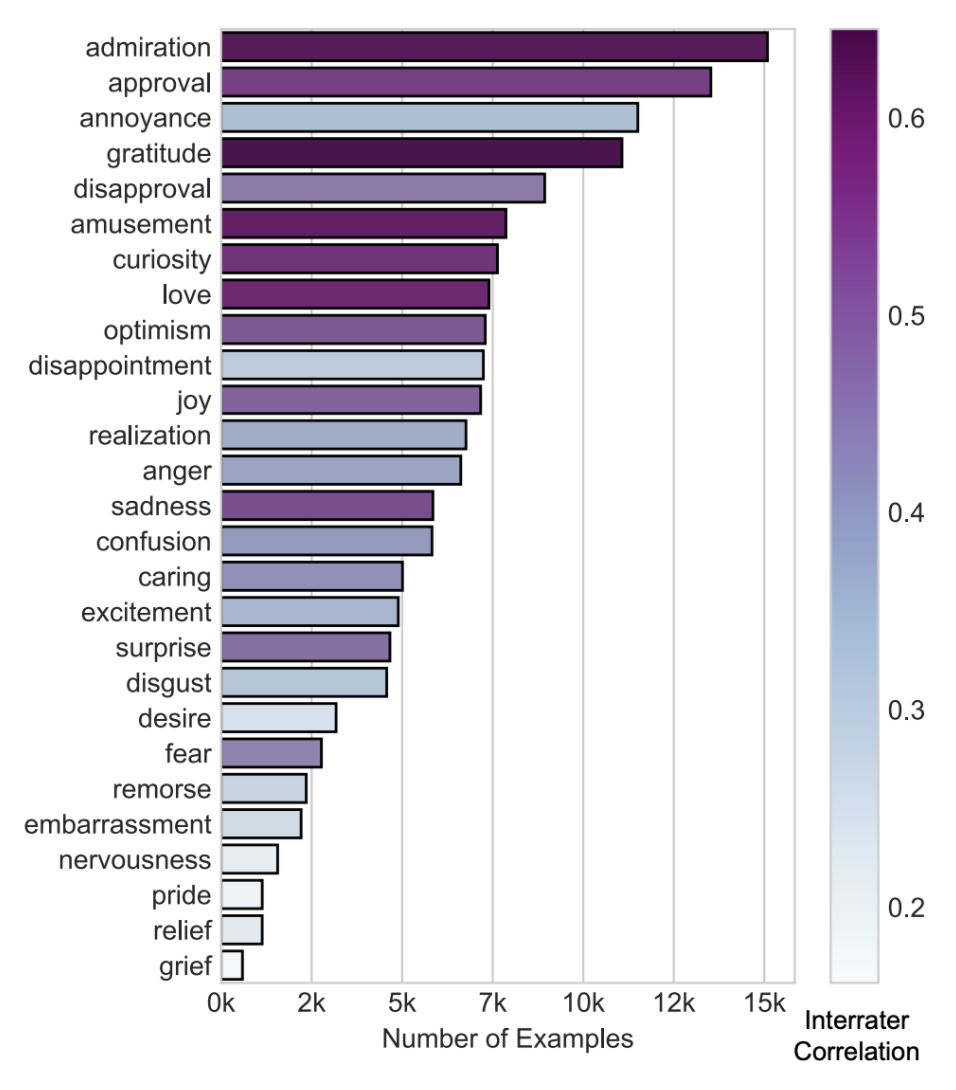
\includegraphics[width=8cm]{labels}
\caption{Frequency of emotion categories in the GoEmotions data set}
\end{figure}

Several measures have been taken to avoid bias. Adult content, racism, sexism and other profanities have been filtered out manually. The comments sources have been restricted to those that are diverse in nature. This was determined through a model created based on a pilot experiment. 

\subsection{Basic Statistics}

In the following we provide an analysis of basic characteristics of the GoEmotions data set. The data set contains sentences with varying lengths, which are evenly distributed between two and 30 words per sentence, and most sentences contain under 200 characters, see figure  \ref{fig:chars_words_dist}. Furthermore, there are a few tokens that occur very often, whereas others occur less frequent, see figure \ref{fig:tokens}. When conducting an analysis of the vocabulary of the data set we identified 65523 unique words before and 18455 after the tokenization.

\begin{figure}[H]
\centering
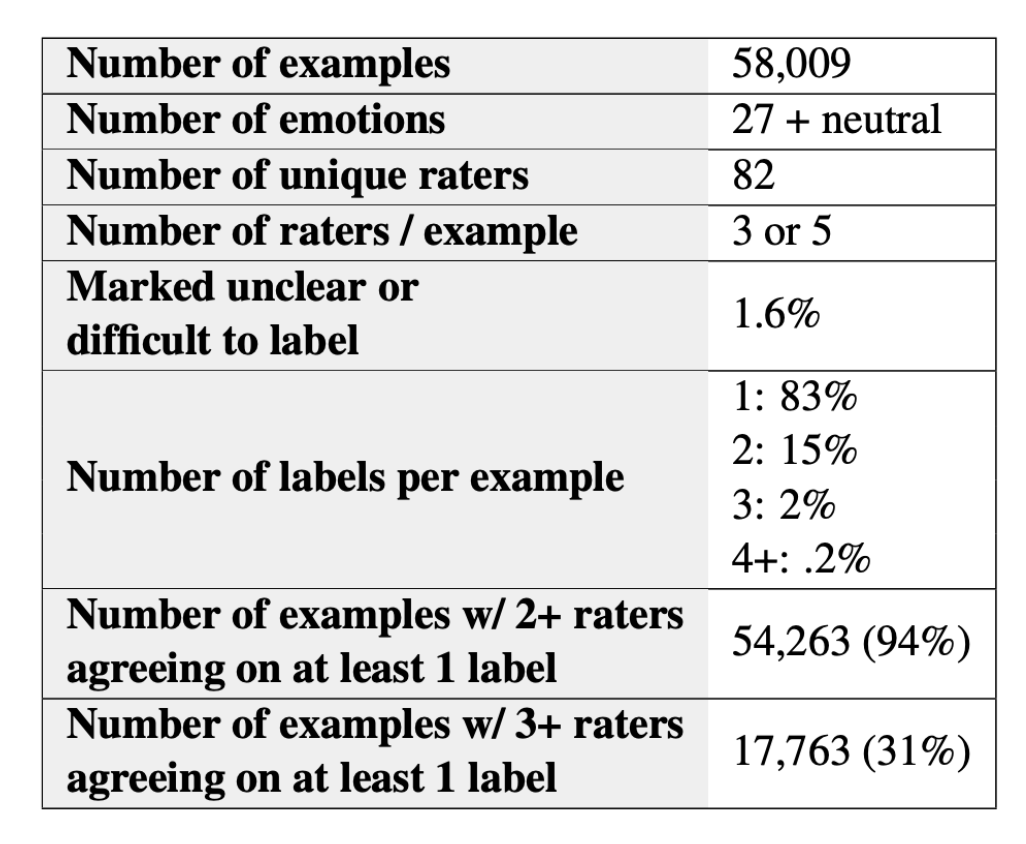
\includegraphics[width=7cm]{statistics}
\caption{Basic statistics on the data set and the labeling of the raters\footref{goemotions_paper}}
\label{fig:statistics}
\end{figure}

\begin{figure}[H]
\centering
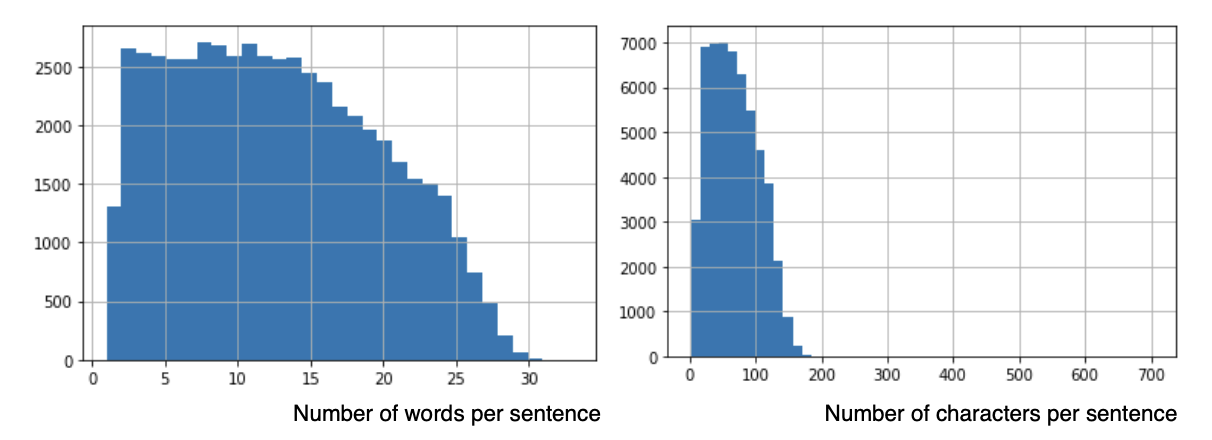
\includegraphics[width=15cm]{chars_words_dist}
\caption{Distribution of the number of words per sentence on the left, for which all frequencies were capped at the median frequency[12] and down-sampled to create the data set. On the right the distribution of the number of characters per sentence split on white space is visualized.}
\label{fig:chars_words_dist}
\end{figure}

\begin{figure}[H]
\centering
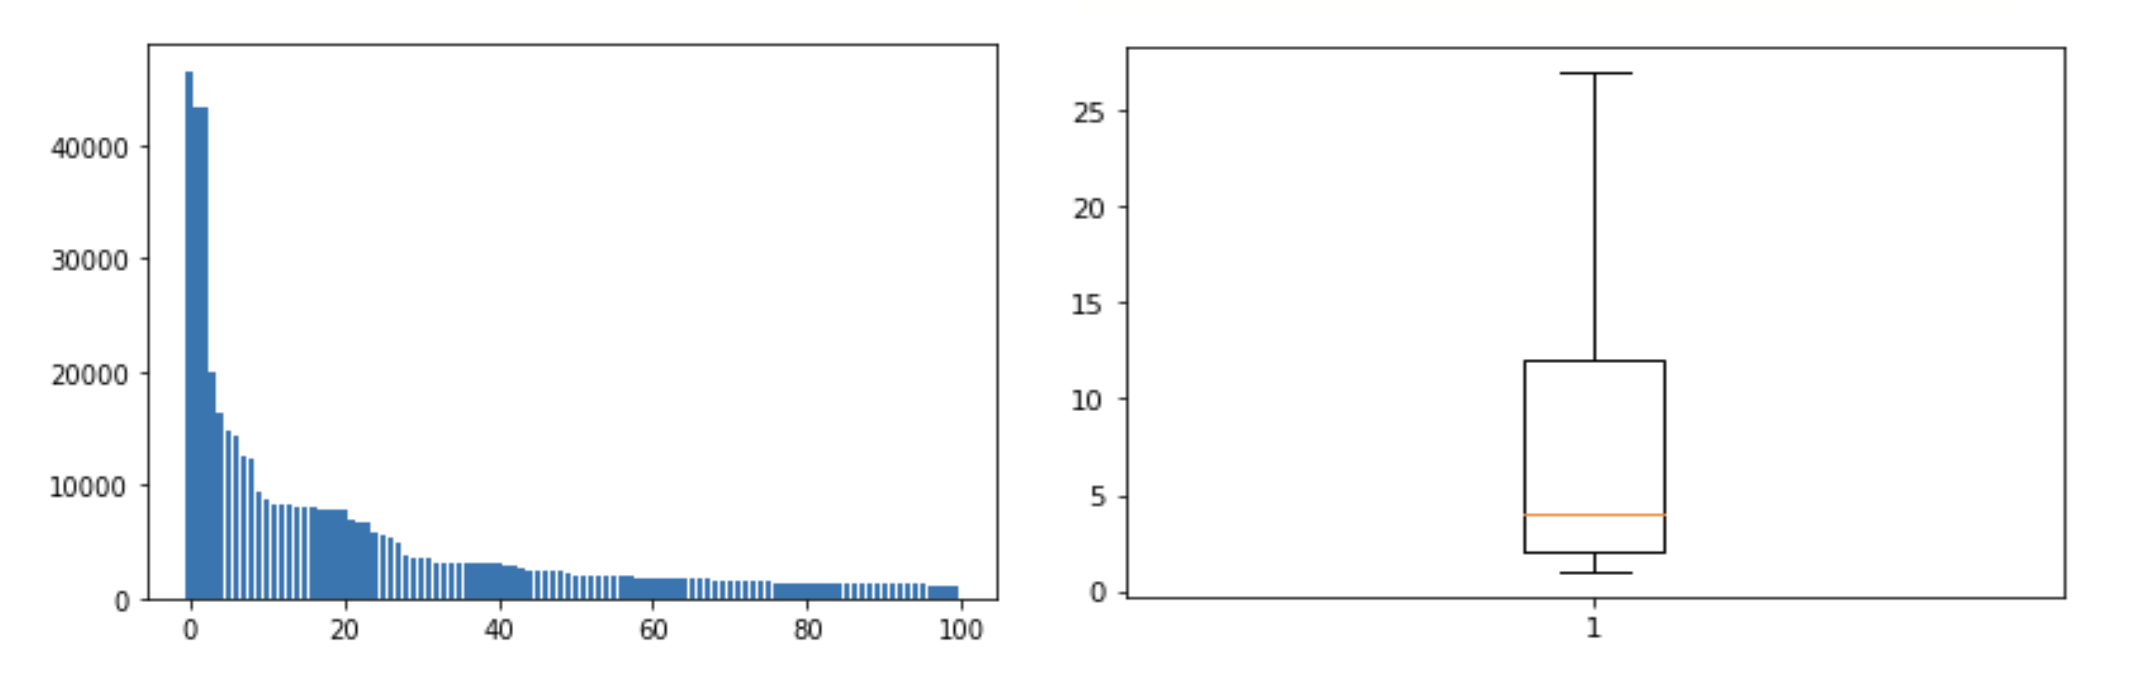
\includegraphics[width=15cm]{tokens}
\caption{Token frequency after tokenization (left: top 100, right: boxplot without outliers)}
\label{fig:tokens}
\end{figure}

%------------------------------------------------

\section{Simple Linguistic Model}

First we encode the \textit{GoEmotions} data set using the \texttt{AutoTokenizer} from \textit{transformers}. The data is then trained using a case-sensitive  \texttt{DistilBertForSequenceClassification} model, which is pretrained on English corpora. As we aim to predict multiple emotions, we face a multi-label task and adapt our loss function accordingly.

The current state of our model can already successfully predict emotions for many dialogue snippets, as listed in table \ref{tab:positive-examples}. However, there are also texts for which the model fails to correctly predict their underlying emotions. Some of such examples, which are falsely labeled as neutral, are listed in table \ref{tab:negative-examples}. From the first negative example it seems that the model cannot properly deal with white spaces. Also, it fails to properly interpret the ``more'' and the past tense of ``expect'' in the second example. Furthermore, the model cannot process smileys. 

\begin{table}[h]
\begin{center}
\begin{tabular}{ l l l } 
\hline
Text & Detected emotions\\
\hline
OMG! & surprise (0.75), excitement (0.28)\\ 
I'm so happy to see you & joy (0.75)\\ 
Shit & annoyance (0.5), anger (0.29)\\ 
holy shit & surprise (0.48)\\ 
It took me a while to get here and I'm sleepy, but I can finally hug you! & caring (0.38), joy (0.23)\\ 
It took me a while to get here and I'm sleepy, but I can finally kill you! & anger (0.29)\\ 
\hline
\end{tabular}
\caption{\label{tab:positive-examples}Positive model results (Showing all emotions with output $>$ 0.2)}
\end{center}
\end{table}

\begin{table}[h]
\begin{center}
\begin{tabular}{ l l l } 
\hline
Text & Detected emotions\\
\hline
O M G & neutral (0.93)\\ 
I expected a lot more from you & optimism (0.44), neutral (0.38)\\ 
I'm SO HAPPY to see you & neutral (0.6)\\ 
Hi! \emoji{heart-eyes}\emoji{heart-eyes} & neutral (0.6)\\ 
Come on man >:( & neutral (0.95)\\ 
\hline
\end{tabular}
\caption{\label{tab:negative-examples}Negative model results (Showing all emotions with output $>$ 0.2)}
\end{center}
\end{table}

%------------------------------------------------

\section{Next Steps}
Originally, we were planning to analyze chat messages, but obtaining these is very difficult and the unique language used in these would prove to be a challenge. Therefore, we opted to analyze movies and show scripts. Specifically we want to take a look at dialogues of the series \textit{Friends} that are available online. The data set contains a collection of all the conversations that occurred in over 10 seasons.\footnote{Friends data set: \url{https://convokit.cornell.edu/documentation/friends.html}} We can potentially expand our analysis to other data sets as well. Using a fine-tuned model that is able to predict emotions, we want to predict emotions on a per sentence basis. Using these predictions, we want to analyze how emotions differ between characters in general and infer other characteristics such as how often a character switches the tone of a conversation or who starts the most conflicts. 

Our next steps include applying the model on the Friends data set, as well as fine tuning it to make even better predictions. Moreover, we could enable the model to interpret the meaning of emojis. This can be achieved by either by training it on a large text corpus that contains emojis and associated emotions, or by statically mapping emojis to emotions\footnote{Emotion tags for emojis: \url{https://github.com/abushoeb/emotag}}.

%------------------------------------------------

\end{document}
